\documentclass[onecolumn,11pts]{IEEEtran}
\usepackage[utf8]{inputenc}
\usepackage{listings}
\usepackage{xcolor}
\usepackage{url}
\usepackage{hyperref}
\usepackage{graphicx}
\usepackage{anysize}
\usepackage[spanish]{babel}
\marginsize{3.5cm}{2.5cm}{3cm}{3cm} 
\hypersetup{
  colorlinks=false,       % false: boxed links; true: colored links
  pdfborder={0 0 0}       % remove ugly border from links
}


\markboth{Redes de Datos}%
{Informe}
\date{November 2016}

\begin{document}

\begin{titlepage}

\begin{center}
\vspace*{-1in}
\begin{figure}[htb]
\begin{center}

\includegraphics[scale=0.4]{UDP}
\end{center}
\end{figure}
Facultad de Ingeniería y Ciencias\\Escuela de Informática y Telecomunicaciones\\
\vspace*{0.15in}
\vspace*{1in}

\begin{LARGE}
\textbf{Levantamiento de Topología Física y Lógica} \\
\end{LARGE}
\vspace*{1in}
\begin{large}
Profesor: José Perez\\Ayudante: Alexis Inzunza\\07/04/2017
\end{large}
\vspace*{0.3in}
\vspace*{1in}
\begin{large}
\begin{flushright}

Integrantes: \\
Benjamín Alvarez \\ Sebastián Antón \\ Jorge Ramirez \\ Nicolás Reyes\\
\end{flushright}
\end{large}
\end{center}
\end{titlepage}


\tableofcontents % indice de contenidos

\cleardoublepage

\cleardoublepage

\title{Actividades de Laboratorio}

\maketitle



       Para esta actividad identificamos aspectos de la topología física y lógica que está presente en el Laboratorio de Informática de la universidad.
       
\section{IDENTIFICACIÓN DE ELEMENTOS DE RED}

\subsection{Identificación de equipos conectados} 

        El laboratorio de Informática está compuesto por 18 computadores, 17 para los alumnos y 1 para el profesor. Estos están conectados a un switch que se encuentra detrás del computador destinado para los profesores. Los computadores están distribuidos de 2 computadores por mesón, exceptuando 1 computador que está solo al final de una fila. Estos se conectan al switch a través de un cable que conecta al switch con un conector a cada mesón, y este conector tiene dos salidas para poder conectar los dos computadores a la red. Esta forma de conectar los computadores es llamada topología “estrella”.
        
\subsection{Identificar el o los switches de la topología} 

        En el laboratorio hay un switch que conecta a todos los computadores de él y adicional a esto, existe un rack de piso ubicado en el laboratorio de Telemática, que es la estructura superior a la que está conectado el switch del laboratorio de Informática (Fig 1).

\subsection{Identificar hardware de red en general considerando la marca y modelo de los mismos}   

        Los computadores tienen la tarjeta de red Intel(R) PRO/1000 MT, esta tarjeta tiene la particularidad de poder adaptarse a la velocidad que admita la red a la cual está conectado el computador y se auto configura para que los encargados de la red ahorren tiempo en su configuración. Esta tarjeta se conecta a la red mediante un puerto RJ-45 con cables de categoría 5. Su ratio de transferencia de datos es de 10Mbps para red Ethernet, 100Mbps para Fast Ethernet y 1Gbps para Ethernet Gigabit (Fig 2).
        


\subsection{Identificar el tipo de cableado utilizado}

        El tipo de cable utilizado en esta red es el cable categoría 5E, el cual cumple con el estándar de red LAN, el cual es capaz de soportar conexiones de 100 Mbps de velocidad y transmisión de datos y voz de hasta 100 Mhz (Fig 3).

\subsection{Identificar el Patch Panel si lo hubiera}

        El Patch Panel está ubicado en el mismo rack en el que está el switch de la sala, y está situado arriba de este. El Patch Panel cumple con la función de conectar el switch con los cables que van direccionados a los computadores, se conecta el switch al patch panel y este último va conectado con los cables que llegan a los computadores. Se hace esto para ampliar la duración del switch, ya que si queremos conectar o desconectar un cable del switch, los conectores y/o los cables se pueden ir dañando con su uso, por este motivo, el patch panel cumple esa función, ya que en términos monetarios, el Patch Panel es más fácil de reemplazar que el switch (Fig 4).
                

\section{INFORMACIÓN DE LOS DISPOSITIVOS}

        En esta actividad buscamos las direcciones IP y MAC para comprender mejor la red del equipo o dispositivo conectado.
        Para hacer esto usamos el terminal de Ubuntu (En el buscador ingresar “Terminal” y abrir) e ingresamos el comando ifconfig (Fig 5).     
        
        Aquí logramos encontrar que las direcciones IP y MAC del PC de el Laboratorio eran  172.16.32.103 y 40:a8:f0:56:47:8b, respectivamente.
        
        
\section {DIAGRAMA DE RED}
        Por último se nos fue pedido realizar un diagrama de red utilizando algún programa para diagramar redes como Windows Visio, Draw.IO, Cacoo, Edraw, etc.
          En este caso, el diagrama de red será una representación del laboratorio de informática, señalando la topología y los “switch” utilizados, complementando toda la información anterior. A continuación analizaremos el diagrama (Fig 6).

        
        En la parte superior, podemos ver el “switch”, el cual está conectado a los 18 computadores a través de unos conectores (las cajas blancas) que están pegados a la muralla. de esta forma cada computador tiene su propia conexión al switch, de manera que si por algún motivo un pc deja de funcionar, esto no afectaría a los demás ordenadores.
        
\section{Conclusión}
Logramos determinar que el laboratorio cuenta con una topología de estrella, , porque observamos que hay un solo rack del que salen las conexiones a todos los equipos del laboratorio.    Además con los resultados obtenidos de este laboratorio pudimos entender la forma en que los elementos de la red del Laboratorio de Informática de la universidad están cableados de la manera aprendida con las normas estudiadas en clases . También, usando el computador, pudimos revisar tanto las direcciones  IP y MAC ,usando el terminal,  para tener una mayor comprensión de la red.

\newpage

\section{Figuras}
\begin{figure}[h!]
\centering
 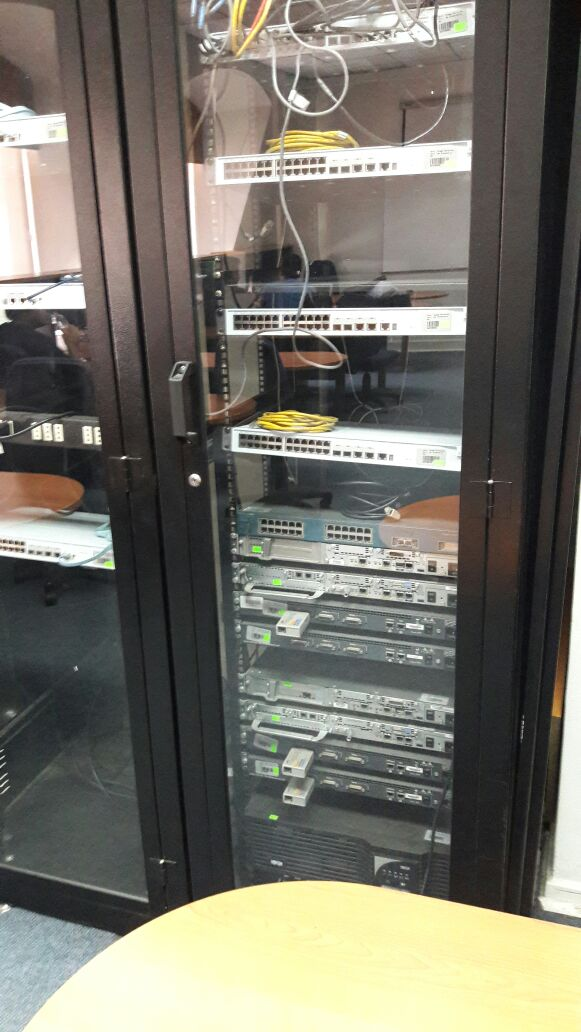
\includegraphics[scale=0.4]{rack}
\caption{Rack de piso}
\label{fig:rack}
\end{figure}

\begin{figure}[h!]
\centering
 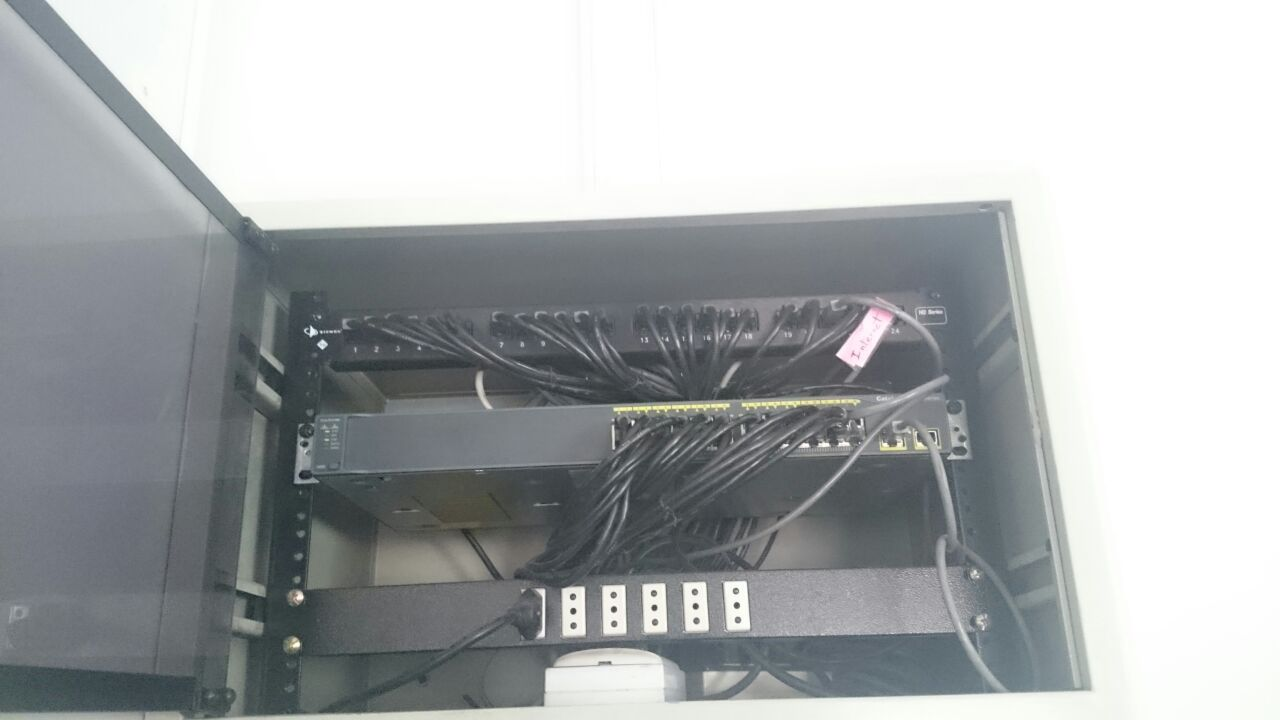
\includegraphics[scale=0.4]{switch}
\caption{Switch Lab. Informática}
\label{fig:switch}
\end{figure}

\begin{figure}[h!]
\centering
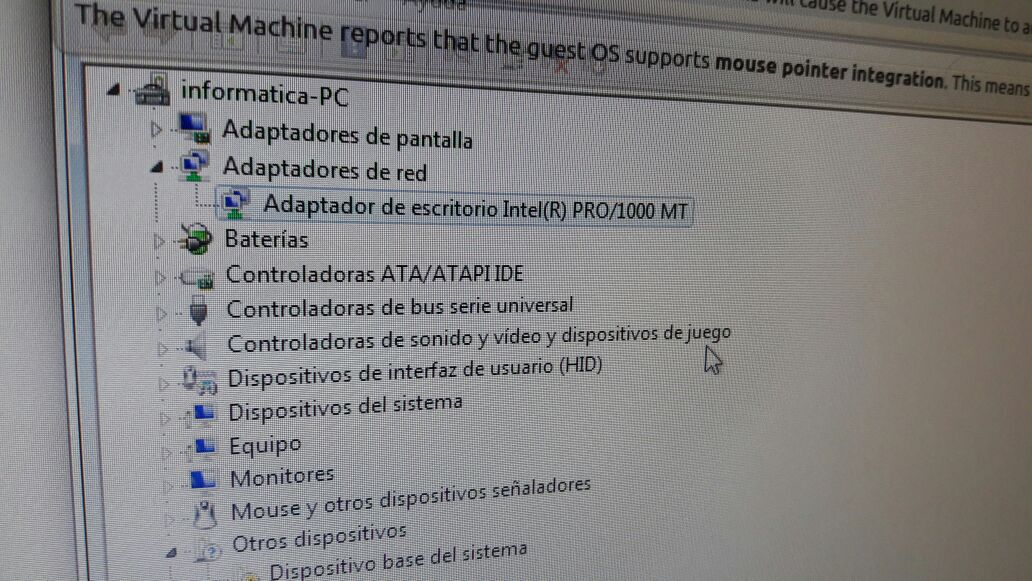
\includegraphics[scale=0.4]{tarjetared}
\caption{Tarjeta red}
\label{fig:tarjeta}
\end{figure}

\begin{figure}[h!]
\centering
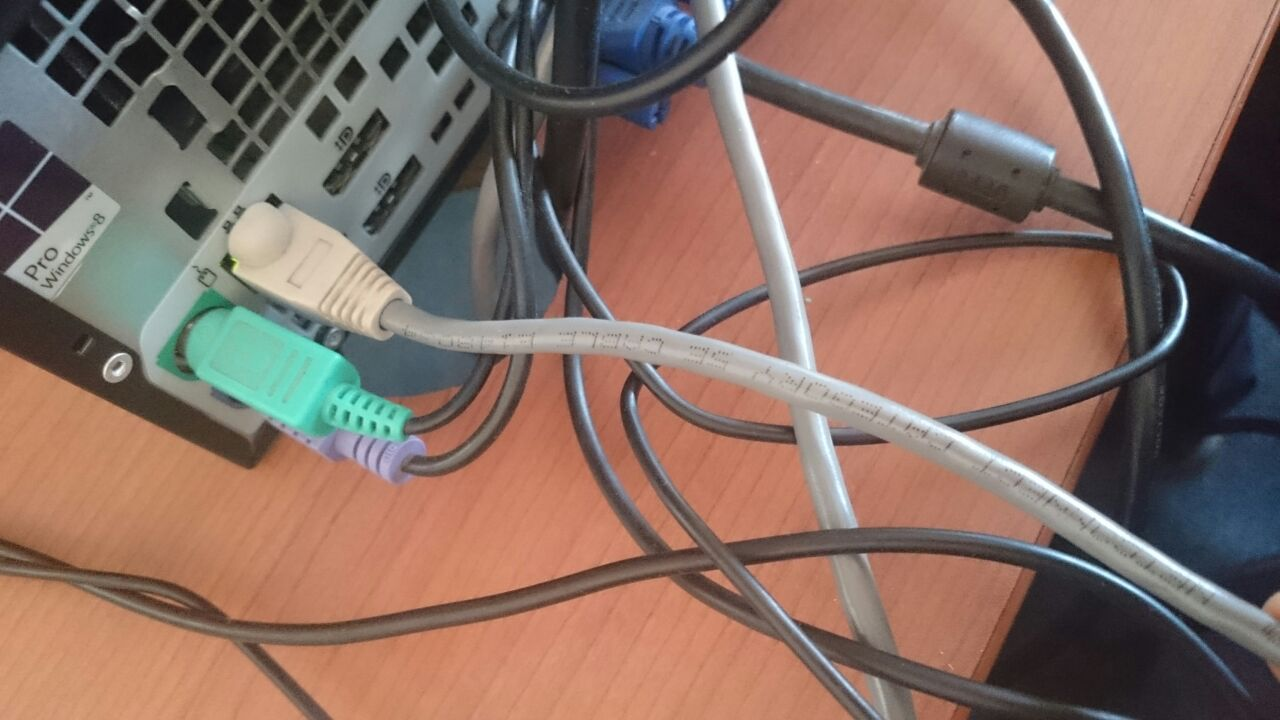
\includegraphics[scale=0.3]{cable5e}
\caption{Cable categoría 5E}
\label{fig:cable red}
\end{figure}

\begin{figure}[h!]
\centering
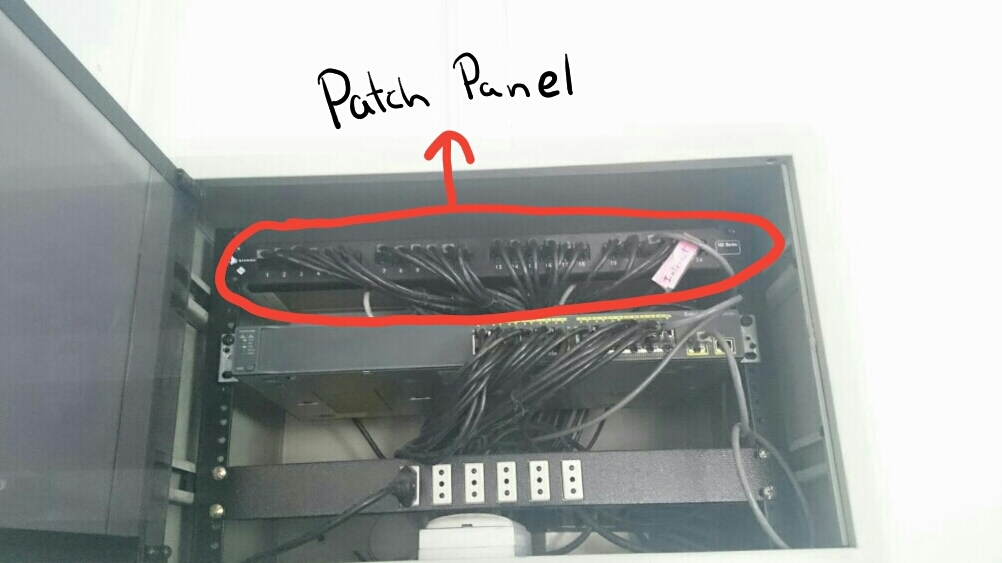
\includegraphics[scale=0.5]{patchpanel}
\caption{Patch Panel}
\label{fig:patch panel}
\end{figure}

\begin{figure}[h!]
\centering
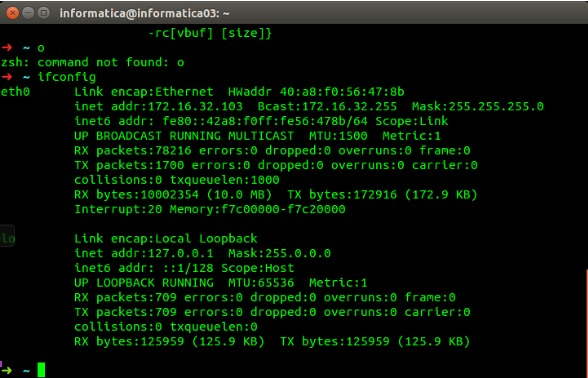
\includegraphics[scale=0.5]{terminal}
\caption{IP y MAC}
\label{fig:terminal}
\end{figure}  

\begin{figure}[h!]
\centering
 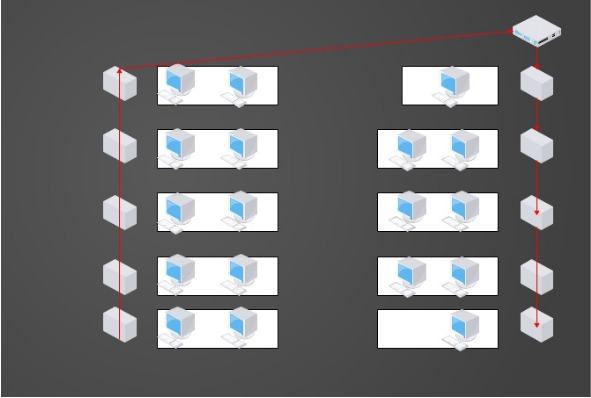
\includegraphics[scale=0.6]{diagrama}
\caption{diagrama Lab. Informática}
\label{fig:diagrama}
\end{figure}


\clearpage

\begin{thebibliography}{15}

\bibitem{mfp}
  Tarjeta de Red Intel Pro 1000 MT Dual Port Server PCI Gigabit Ethernet RJ45,
  \emph{intercompras}
  \url{https://goo.gl/vsqJPL}
  

\end{thebibliography}

\end{document}
